\section{Convolutional Neural Network}

\subsection{Geschichte}

\paragraph{Zellarten} 
Im Jahr 19459 beschrieben die beiden Neurophysiologe Torsten Wiesel und David H. Hubel die sogenannten \emph{simple} und \emph{complex cells}. Sie beschrieben einen groben Zusammenhang dafür wie diese beiden Zellarten bei der Mustererkennung im visuellen Cortex verwendet werden. 

\begin{itemize}
\item Die \emph{simple cells} können einfache Kanten und Balken mit einer bestimmten Orientierung erkennen. Abbildung \ref{fig:gabor_filter} zeigt welche Art von Formen von diesen Zellen erkannt werden können. Ein solche Zelle könnte zum Beispiel in der Lage sein einen Balken am unteren Bildrand als solchen zu erkennen. 

\item Eine \emph{komplexe} ist ebenfalls dazu in der Lage diese Formen zu erkennen allerdings mit dem Zusatz, dass sie in der Lage ist diese Konstellation von Formen auch an verschiedenen Positionen des Bildes zu erkennen. Bezogen auf das Beispiel vom letzten Punkt, könnte diese Zellart auch in der Lage sein, solche Balken in der Mitte oder am oberen Rand des Bildes zu erkennen. Diese Eigenschaft der Positionsunabhängigkeit eines Musters wird \emph{spatial invariance} genannt (zu deutsch \glqq räumliche Invarianz \grqq ).
\end{itemize}

\begin{figure}[!htb]
	\centering
	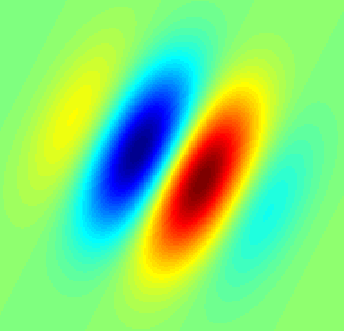
\includegraphics[width=.5\linewidth]{img/gabor_filter}
	\mycaption{Simple Cell - Beispiel}{cnnHistory}
	\label{fig:gabor_filter}
\end{figure}

Einige Jahre später (1962), beschrieben die beiden Wissenschaftler wie solche komplexen Zellen die Eigenschaft der \emph{partial invariance} erreichen. Diese Zellen summieren die Ausgaben von mehreren \emph{simple cells} auf. Diese Zellen sind auf die gleichen Formen spezialisiert, analysieren jedoch jeweils einen unterschiedlchen Teil des Bildes (englisch \emph{receptive fields}, siehe Abbildung \ref{fig:simpleVsComplex}). So kann zum Beispiel eine komplexe Zelle horizonale Balken an mehreren Positionen im Bild erkennen indem sie auf die unterschiedlichen Ausgabewerte von mehreren simplen Zellen zurückgreift und diese aufaddiert. Diese Herangehensweise des Herunterbrechens einer komplexen Aufgabe in mehrere einfachere Aufgaben ist ein wesentliches Merkmal aller neuronalen Netze sowie der menschlichen Wahrnehmung im visuellen Kortex. 

\begin{figure}[!htb]
	\centering
	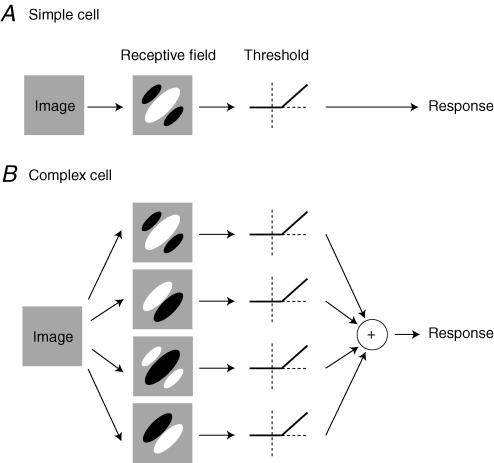
\includegraphics[width=.6\linewidth]{img/simpleVsComplex}
	\mycaption{Vergleich  - Simple und Complex Cell}{simpleComplexCell}
	\label{fig:simpleVsComplex}
\end{figure}

In den 1980er entwickelte Dr. Kunihiko Fukushima das Modell von Hubel und Wiesel weiter indem er ein mathematisches Modell mit den beiden Typen \emph{S-Cells} und \emph{C-Cells} einführte. Die S-Cells befinden sich jeweils in der ersten Schicht des Modells und sind mit den C-Cells verbunden. 

\paragraph{Erkennung von Handschrift}
Einer der Pioniere auf dem Gebiet ist der französische Informatiker Yann LeCun. In einer Ausarbeitung wie ein simples CNN Modell in der Lage ist handschriftliche Ziffern zu erkennen. Sein Modell verwendet wie schon angedeutet die Eigenschaft mit einfach Formen komplexere zu bilden und somit die Ziffern zu erkennen. Um sein Modell zu trainieren verwendete der die \emph{MNIST database of handwritten digits}. Diese Datenbank enthält 




\subsection{Funktionsweise}
\blindtext
